\documentclass[a4paper,english,12pt]{article}
\usepackage{%
	amsmath,%
	amsfonts,%
	amssymb,%
	amsthm,%
	hyperref,%
	url,%
	latexsym,%
	epsfig,%
	graphicx,%
	psfrag,%
	subfigure,%	
	color,%
	tikz,%
	pgf,%
	pgfplots,%
	pgfplotstable,%
	pgfpages,%
	proofs%
}

\usepgflibrary{shapes}
\usetikzlibrary{%
  arrows,%
	backgrounds,%
	chains,%
	decorations.pathmorphing,% /pgf/decoration/random steps | erste Graphik
	decorations.text,%
	matrix,%
  positioning,% wg. " of "
  fit,%
	patterns,%
  petri,%
	plotmarks,%
  scopes,%
	shadows,%
  shapes.misc,% wg. rounded rectangle
  shapes.arrows,%
	shapes.callouts,%
  shapes%
}

\theoremstyle{plain}
\newtheorem{thm}{Theorem}[section]
\newtheorem{lem}[thm]{Lemma}
\newtheorem{prop}[thm]{Proposition}
\newtheorem{cor}[thm]{Corollary}

\theoremstyle{definition}
\newtheorem{defn}[thm]{Definition}
\newtheorem{conj}[thm]{Conjecture}
\newtheorem{exmp}[thm]{Example}
\newtheorem{assum}[thm]{Assumptions}

%\theoremstyle{remark}
\newtheorem{rem}{Remark}
\newtheorem{note}{Note}

\makeatletter
\def\th@plain{%
  \thm@notefont{}% same as heading font
  \itshape % body font
}
\def\th@definition{%
  \thm@notefont{}% same as heading font
  \normalfont % body font
}
\makeatother
\date{}
%\usepackage[T1]{fontenc}
%\PassOptionsToPackage{normalem}{ulem}
%\usepackage{ulem}

%%%%%%%%%%%%%%%%%%%%%%%%%%%%%% LyX specific LaTeX commands.
%\pdfpageheight\paperheight
%\pdfpagewidth\paperwidth
%\makeatother

%\usepackage{babel}

\begin{document}

\title{Lecture 13: Basis for a Topology}
\author{}
\maketitle


\section{Basis for a Topology}

\begin{lem} \label{basis_alternate_defn_2}
 Let $(X, \T)$ be a topological space. Suppose that $\C$ is a collection of open sets of $X$ such that for each open set $U$ of $X$
 and each $x$ in $U$, there is an element $C \in \C$ such that $x \in  C \subset U$. Then $\C$ is the basis for the topology of $X$.
\end{lem}
\begin{proof}
In order to show that $\C$ is a basis, need to show that $\C$ satisfies the two properties of basis. To show the first property, let $x$ be an element of the open 
set $X$. Now, since $X$ is open, then, by hypothesis there exists an element $C$ of $\C$ such that $x \in C \subset X$. Thus $\C$ satisfies the first property of 
basis. 

To show the second property of basis, let $x \in X$ and $C_{1}, C_{2}$ be open sets in $\C$ such that $x \in C_{1}$ and $x \in C_{2}$. This implies that 
$C_{1} \cap C_{2}$ is also an open set in $\C$ and $x \in C_{1} \cap C_{2}$. Then, by hypothesis, there exists an open set $C_{3} \in \C$ such that
$x \in C_{3} \subset C_{1} \cap C_{2}$. Thus, $\C$ satisfies the second property of basis too and hence, is indeed a basis for the topology on $X$.
\end{proof}

On many occasions it is much easier to show results about a topological space by arguing in terms of its basis. For example, to determine whether one 
topology is finer than the other, it is easier to compare the two topologies in terms of their bases.

\begin{lem} \label{basis_fineness}
 Let $\B$ and $\B^{'}$ be basis for topologies $\T$ and $\T^{'}$, respectively, on $X$. Then, the following are equivalent:
 \begin{enumerate}
  \item $\T^{'}$ is finer than $\T$
  \item For each $x \in X$  and each basis element $B \in \B$ containing $x$, there is a basis element $B^{'} \in \B^{'}$ such that $x \in B^{'} \subset B$.
 \end{enumerate}
\end{lem}
\begin{proof}
 ($2$) $\implies$ ($1$) We need to show that for any open set $U \subset \T$, its also holds that $U \in \T^{'}$. Let $x$ be an arbitrary element of set $U$. Since 
 $\B$ generates $\T$, there exists $B \in \B$ such that $x \in B \subset U$. Then, from (2), there exists $B^{'} \in \B^{'}$ such that $x \in B^{'} \subset B \subset U$.
 Since $x$ is arbitrary, $U \in \T^{'}$ holds. 
 
 ($1$) $\implies$ ($2$) Let $x \in X$ and $B$ be an element of $\B$ containing $x$. Since $\B$ generates $\T$, it holds that $B \in \T$. Then, by hypothesis, it also 
 holds that $B \in \T^{'}$. Now, since $\B^{'}$ is a basis for $\T^{'}$ and $B$ in an open set in $\T^{'}$, there exists a set $B^{'} \in \B^{'}$ such that 
 $x \in B^{'} \subset B$ and we are done.
\end{proof}

A basis $\B$ can be seen as a set of 'building blocks/sets' which can generate any open set in the topology $\T_{\B}$ generated by $\B$. By taking 
arbitrary union or finite intersection of the basis elements, any open set in $\T_{\B}$ can be realized. A useful analogy is to see a topological space 
as a truckload full of gravel. Think of the pebbles as the basis elements of the topology; after the pebbles are smashed to dust, the dust particles are the
basis elements of new topology. The new topology is finer than the old one, and each new dust particle was contained inside a pebble, as Lemma \ref{basis_fineness} states.

\begin{figure}[hhhh]
\centering
 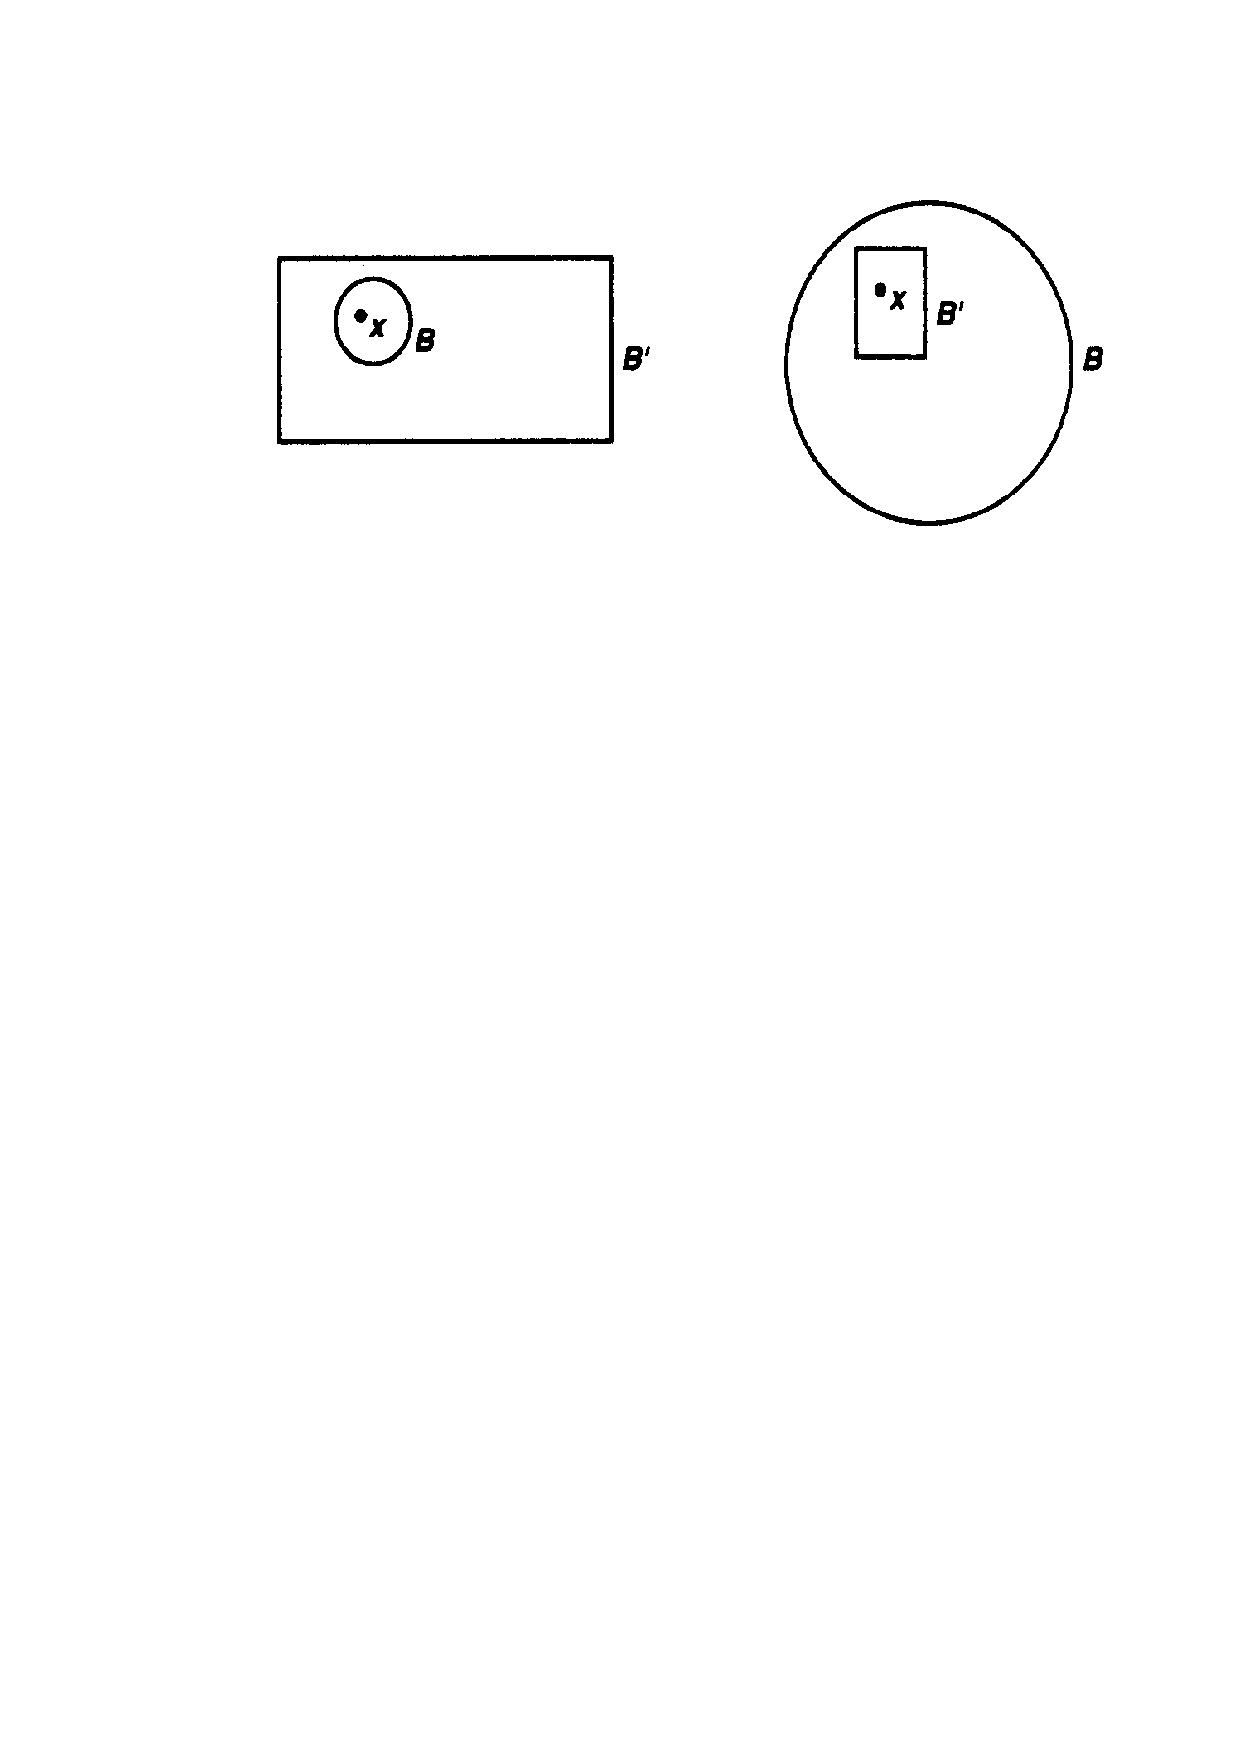
\includegraphics[height=2.0in]{Figures/BasisCompare.pdf}
	\caption{}
 \label{Fig:CompareBasis}
\end{figure}
\begin{exmp}
The collection $\B$ of all circular regions in the plane generates the same topology as the collection $\B^{'}$ of all the rectangular regions. Figur~\ref{Fig:CompareBasis} illustrates the proof. For each element $x$ of an arbitrary circular region in $\B$, there always exists a rectangular region in $\B^{'}$ containing $x$ which fits within the said circular region and vice versa. 
\end{exmp}

We now define three topologies on real line $\R$, all of which are of interest.

\begin{defn}[Standard topology]
If $\B$ is the collection of all open intervals in the real line, 
\begin{equation}
 (a, b) = \{ x | a < x < b\} \nonumber,
\end{equation}
the topology generated by $\B$ is called the \textbf{standard topology} on the real line. Whenever, we consider $\R$, we shall suppose it is given this topology 
unless stated otherwise.
\end{defn}

\begin{defn}[Lower limit topology]
If $\B^{'}$ is the collection of all half open intervals in the real line, 
\begin{equation}
 [a, b) = \{ x | a \leq x < b\} \nonumber,
\end{equation}
the topology generated by $\B^{'}$ is called the \textbf{lower limit topology} on $\R$. When, $\R$ is given the lower limit topology, we denote it by 
$\R_{l}$. Thus, in $\R_{l}$, half open intervals of the form $[a, b)$ for $a, b \in \R$ are open sets.
\end{defn}

\begin{defn}[K - topology]
Let $K$ denote the set of all numbers of the form $\frac{1}{n}$ for $n \in \Z_{+}$, and let $\B^{''}$ be the collection of all intervals $(a, b)$ 
along with all sets of the form $(a, b) \backslash K$. The topology generated by $\B^{''}$ will be called the $K-topology$ on $\R$. When $\R$ is given this topology, we denote it by $\R_{K}$. 
\begin{equation*}
 [a, b) = \{ x | a \leq x < b\},
\end{equation*}
the topology generated by $\B^{'}$ is called the \textbf{lower limit topology} on $\R$. In other words, $\B^{''} = \B \cup \{ (a, b) \backslash K, \forall
a, b \in \R \}$, where $\B$ is the set of all open intervals in $\R$. 
When, $\R$ is given the lower limit topology, we denote it by $\R_{l}$.
\end{defn}


\begin{lem}
The topologies of $\R_{l}$ and $\R_{K}$ are strictly finer that the topology on $\R$, but are not comparable with each other.
\end{lem}
\begin{proof}
To show that a topology $\R_{l}$ is finer that of $\R$, let $x \in (a, b)$, where $(a, b)$ is an arbitrary element of the basis of $\R$. Then, for sufficiently large $n \in \Z_{+}$, we can always construct the half open interval $[a + \frac{1}{n}, b) \subset (a,b)$ (an element of the basis of $\R_{l}$), such that it contains $x$. On the other hand, given a basis element $[a, b)$ for $\R_{l}$, there exists no open interval in $\R$ which contains $a$ but is still lies in $[a,b)$. Hence, the topology $\R_{l}$ is strictly finer than $\R$.
\end{proof}

\begin{defn} [Subbasis]
A \textbf{sub-basis} $\mathcal{S}$ for a topology on $X$ is a collection of subsets of $X$ whose union equals $X$. The \textbf{topology generated by the sub-basis $\mathcal{S}$} is defined to be the collection $\T$ of all unions of finite intersections of elements of $\mathcal{S}$.
\end{defn}

Let us check if the topology $\T$ generated by sub-basis $\mathcal{S}$ as described above satisfies the properties of a valid topology or not.
Rather than using the standard definition of topology, instead we will show first that if $\B$ is the collection of all finite intersections of the elements of $\mathcal{S}$, then $\B$ is a basis. Then, the union of elements of $\B$ will indeed be a topology (as union of elements of basis gives the topology itself).

Given $x \in X$, from definition of sub-basis $\mathcal{S}$, $x$ belongs to an element of $\mathcal{S}$, and hence $x$ belongs to an element of $\B$. So, the first condition of basis is satisfied. To check the second condition, let $B_{1} = S_{1} \cap \dots \cap S_{m}$ and $B_{2} = S_{1}^{'} \dots S_{n}^{'}$ be two elements of $\B$. Then, their intersection $B_{1} \cap B_{2} = (S_{1} \cap \dots \cap S_{m})  \cap (S_{1}^{'} \dots S_{n}^{'})$ is also a finite intersection of elements of $\mathcal{S}$, so it belongs to $\B$. 

\begin{exmp}
\begin{enumerate}[i)]
Consider the set $A = (-1, 1)$ of real numbers in the usual order. Assuming the fact that the real numbers have the least upper bound property, it follows that the set $A$ has the least upper bound property. Any subset of $A$ having an upper bound in $A$ should also have least upper bound property. 
\end{enumerate}
\end{exmp}

\section{Order Topology}
Given a collection of sets, we may want to define an order relation between any two member sets. An order relation can provide the necessary framework for introducing the notion of \textbf{distance} in a very abstract sense. A very crude example is to consider three real number $a, b$ and $c$ such that $b$
is greater than $a$, and $c$ is greater than $b$. In this example, "greater than" is a type of order relation. It is easy to see that $c$ is not only greater than $a$, but also $c$ is \textbf{farther} from $a$ compared to $b$. This is a fine example of how an order relation can induce much richer mathematical entities such as distances, intervals, neighborhoods etc.  

If $X$ is a simply ordered set, there is a standard topology for $X$, defines using the order relation. It is called the $\emph{order topology}$.

Suppose that $X$ is a set having a simple order relation $<$. Given elements $a$ and $b$ of $X$ such that $a < b$. there are four subsets of $X$ that are the intervals determined by $a$ and $b$. They are:
\begin{enumerate}[a)]
\item Open interval: $(a, b) = \{ x\; | \: a < x < b  \}$
\item Half open interval: $[a, b) = \{ x\; | \: a \le x < b  \}$
\item Half open interval: $(a, b] = \{ x\; | \: a < x \le b  \}$
\item Closed interval: $[a, b] = \{ x\; | \: a \le x \le b  \}$
\end{enumerate} 

\end{document}
